\section{Adjusting the Parameters}
\label{sec:add.parameters}

\hl{
	The fixed parameters in the archetypal are $a_L = 4, b_L = -\frac{1}{2},$ and $g_R\left(\frac{1}{2}\right) = \frac{1}{2} + \frac{1}{40}$.
	\hl{O}nly the branches $f_\A$ and $f_\C$ are not monotonously increasing.
	Of the three fixed parameters, $a_L$ and $b_L$ influence the shape of the branches $f_\A$ and $f_\C$.
	These parameters are adjusted to make the branches $f_\A$ and $f_\C$ monotonously increasing.
	The new parameter values are $a_L = 1$ and $b_L = \frac{1}{2}$.
}
\hl{The new shape of the function can be seen in} \Cref{fig:add.arch.new}, \hl{now all branches are monotonously increasing}.
\hl{
	We will refer to this model as the piecewise-increasing archetypal model.
}

\Cref{fig:add.arch.new.period} \hl{shows a 2D scan of the periods associated with parameter regions in the archetypal model with these new values for the fixed parameters stated above}.
\hl{
	In this scan, we can see that the ``type B'' parameter regions disappeared and ``type A'' parameter regions of the same chain seem to start overlapping.
	Also, in between the chains there are now small parameter regions with much higher periods.
	These structures look like \glsentrylong{pa} structures.
	And indeed, it is plausible for \gls{pa} structures to emerge in such a map.
	\Citeauthor{simpson2018saw} demonstrated in his work \cite{simpson2018saw} that a \gls{pws} circle map with two linear and increasing branches can exhibit \gls{pa}.
}
\Cref{fig:add.saw} \hl{shows this map called skew sawtooth next to the piecewise-increasing archetypal model map}.
\hl{
	The skew sawtooth map is continuous while the piecewise-increasing archetypal model map is not.
	And the piecewise-increasing archetypal map has quadratic branches while all branches in the skew sawtooth map are linear.
}
\hl{But they are somewhat similar as we can see in the comparison in} \Cref{fig:add.saw.vs.arch}.

\hl{
	In the following sections these structures are explored.
	They are referred to as \gls{pal} structures.
}
But first, we will take a closer look at how the bifurcations structures change when adjusting the parameters $a_L$ and $b_L$ to make the branches $f_\A$ and $f_\C$ increasing.

\begin{figure}
	\centering
	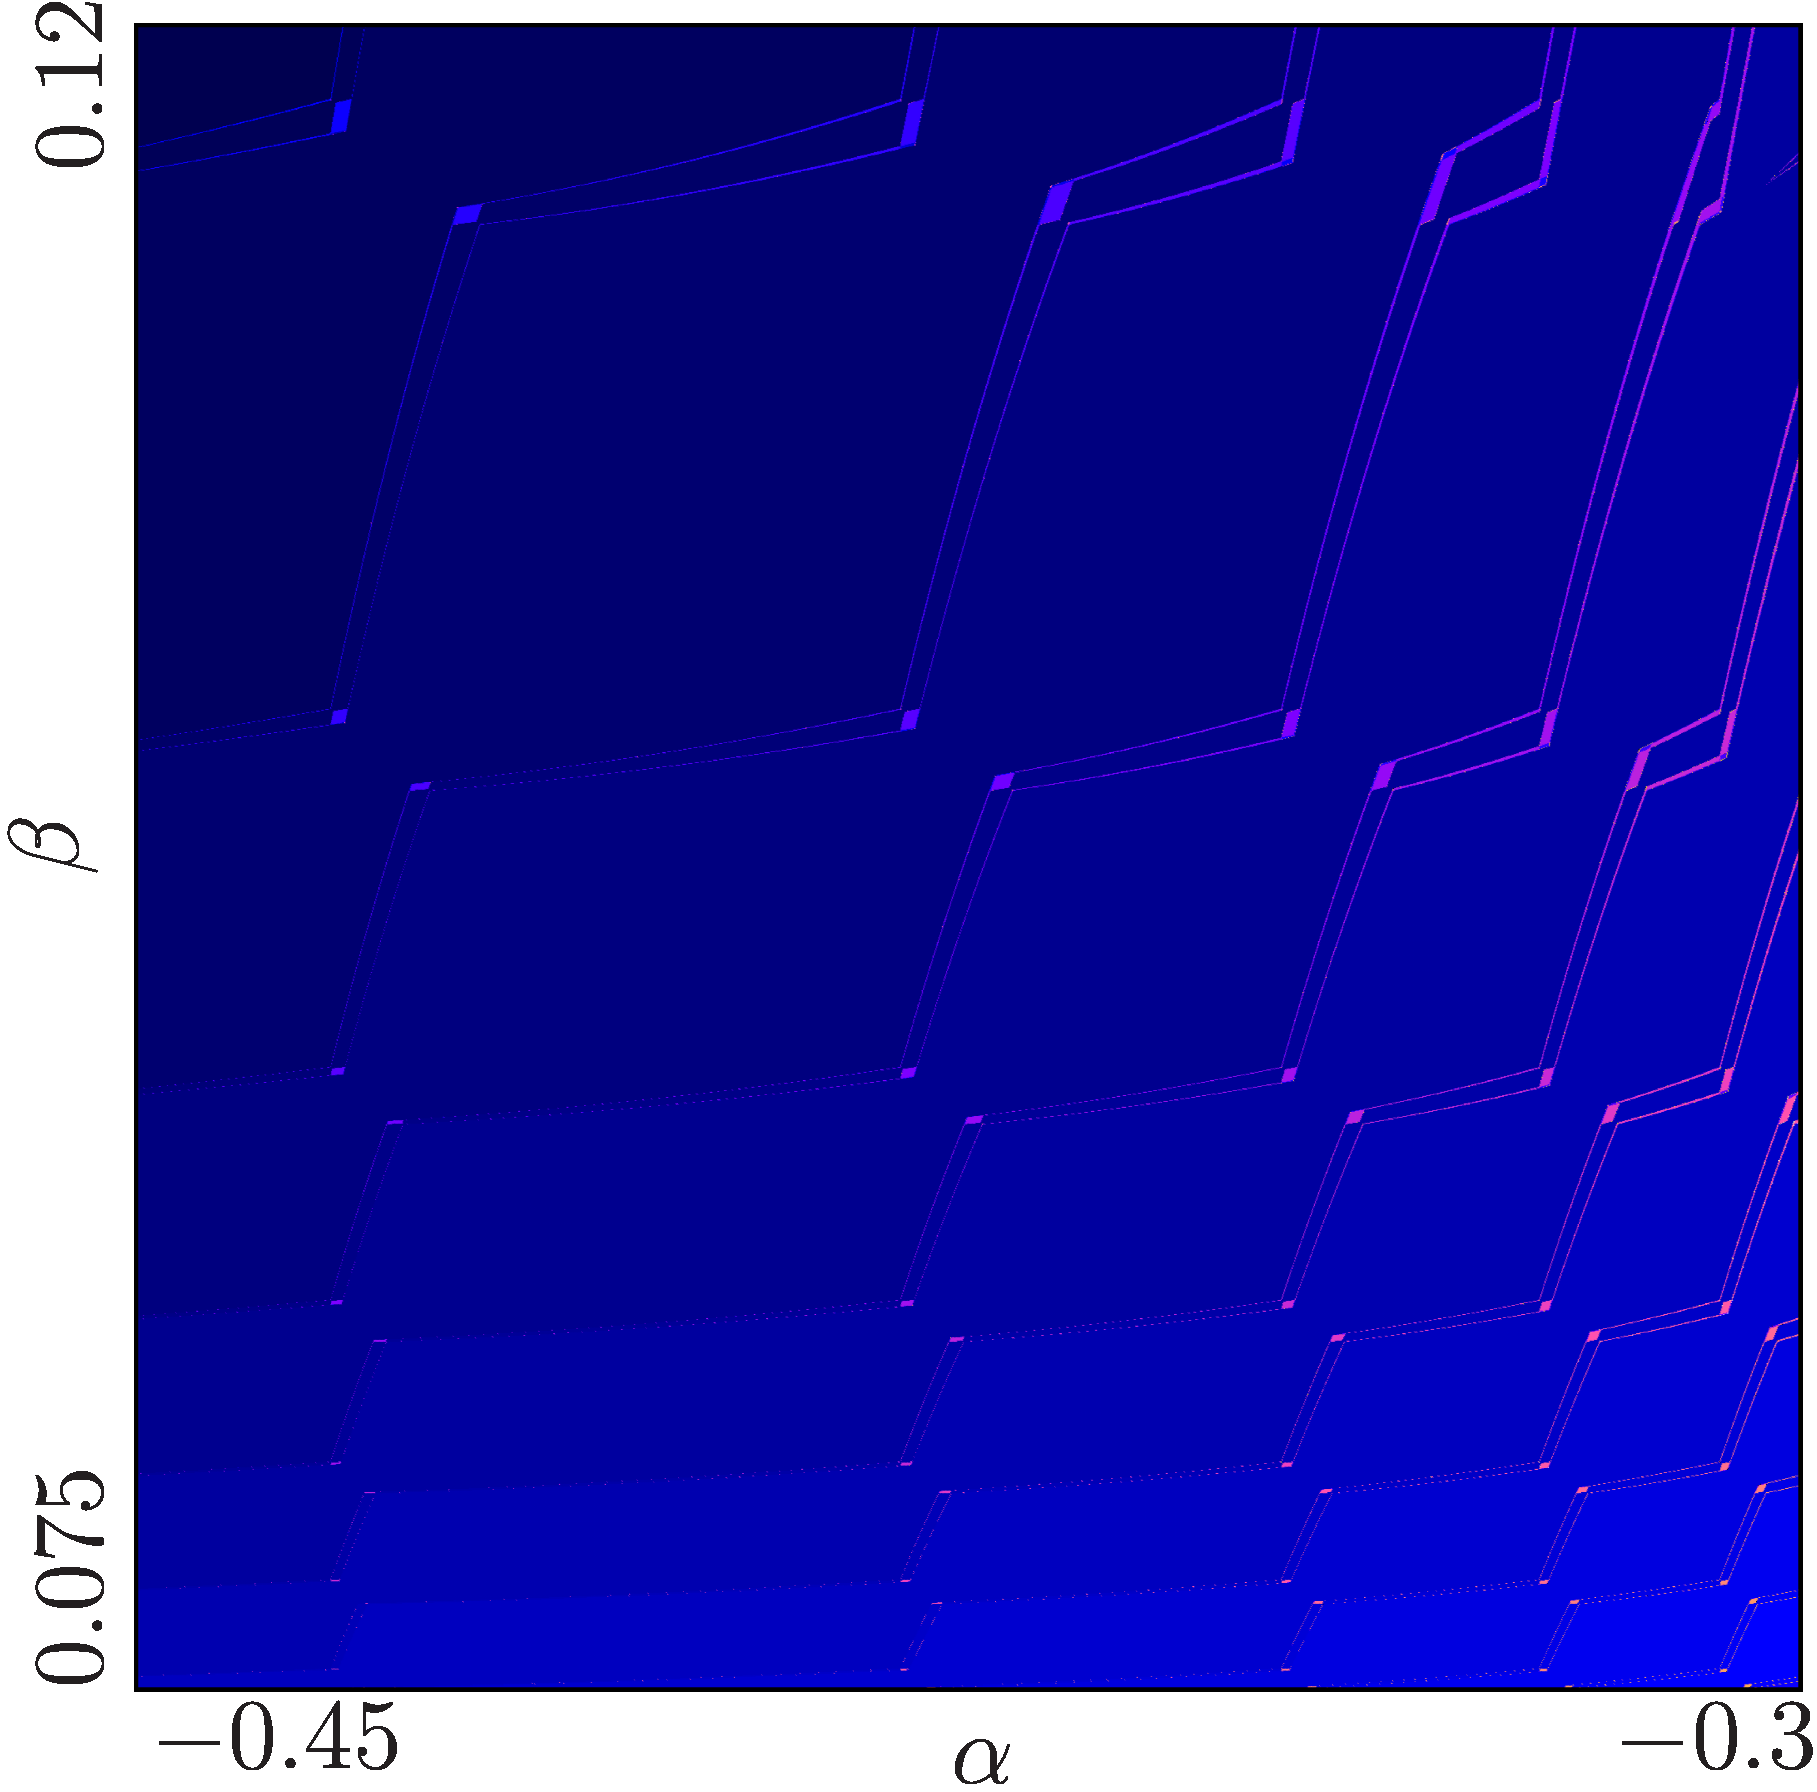
\includegraphics[width=.6 \textwidth]{../Figures/7/7.1/result.png}
	\caption[2D period scan of the piecewise-increasing increasing archetypal model]{
		2D period scan of the piecewise-increasing increasing archetypal model.
		With the fixed parameters $a_L = 1, b_L = \frac{1}{2},$ and $g_R\left(\frac{1}{2}\right) = \frac{1}{2} + \frac{1}{40}$.
		The parameters $\alpha = g_R\left(\frac{1}{4}\right)$ and $\beta = c_L$ are varied.
	}
	\label{fig:add.arch.new.period}
\end{figure}

\begin{figure}
	\centering
	\subfloat[Skew sawtooth map]{
		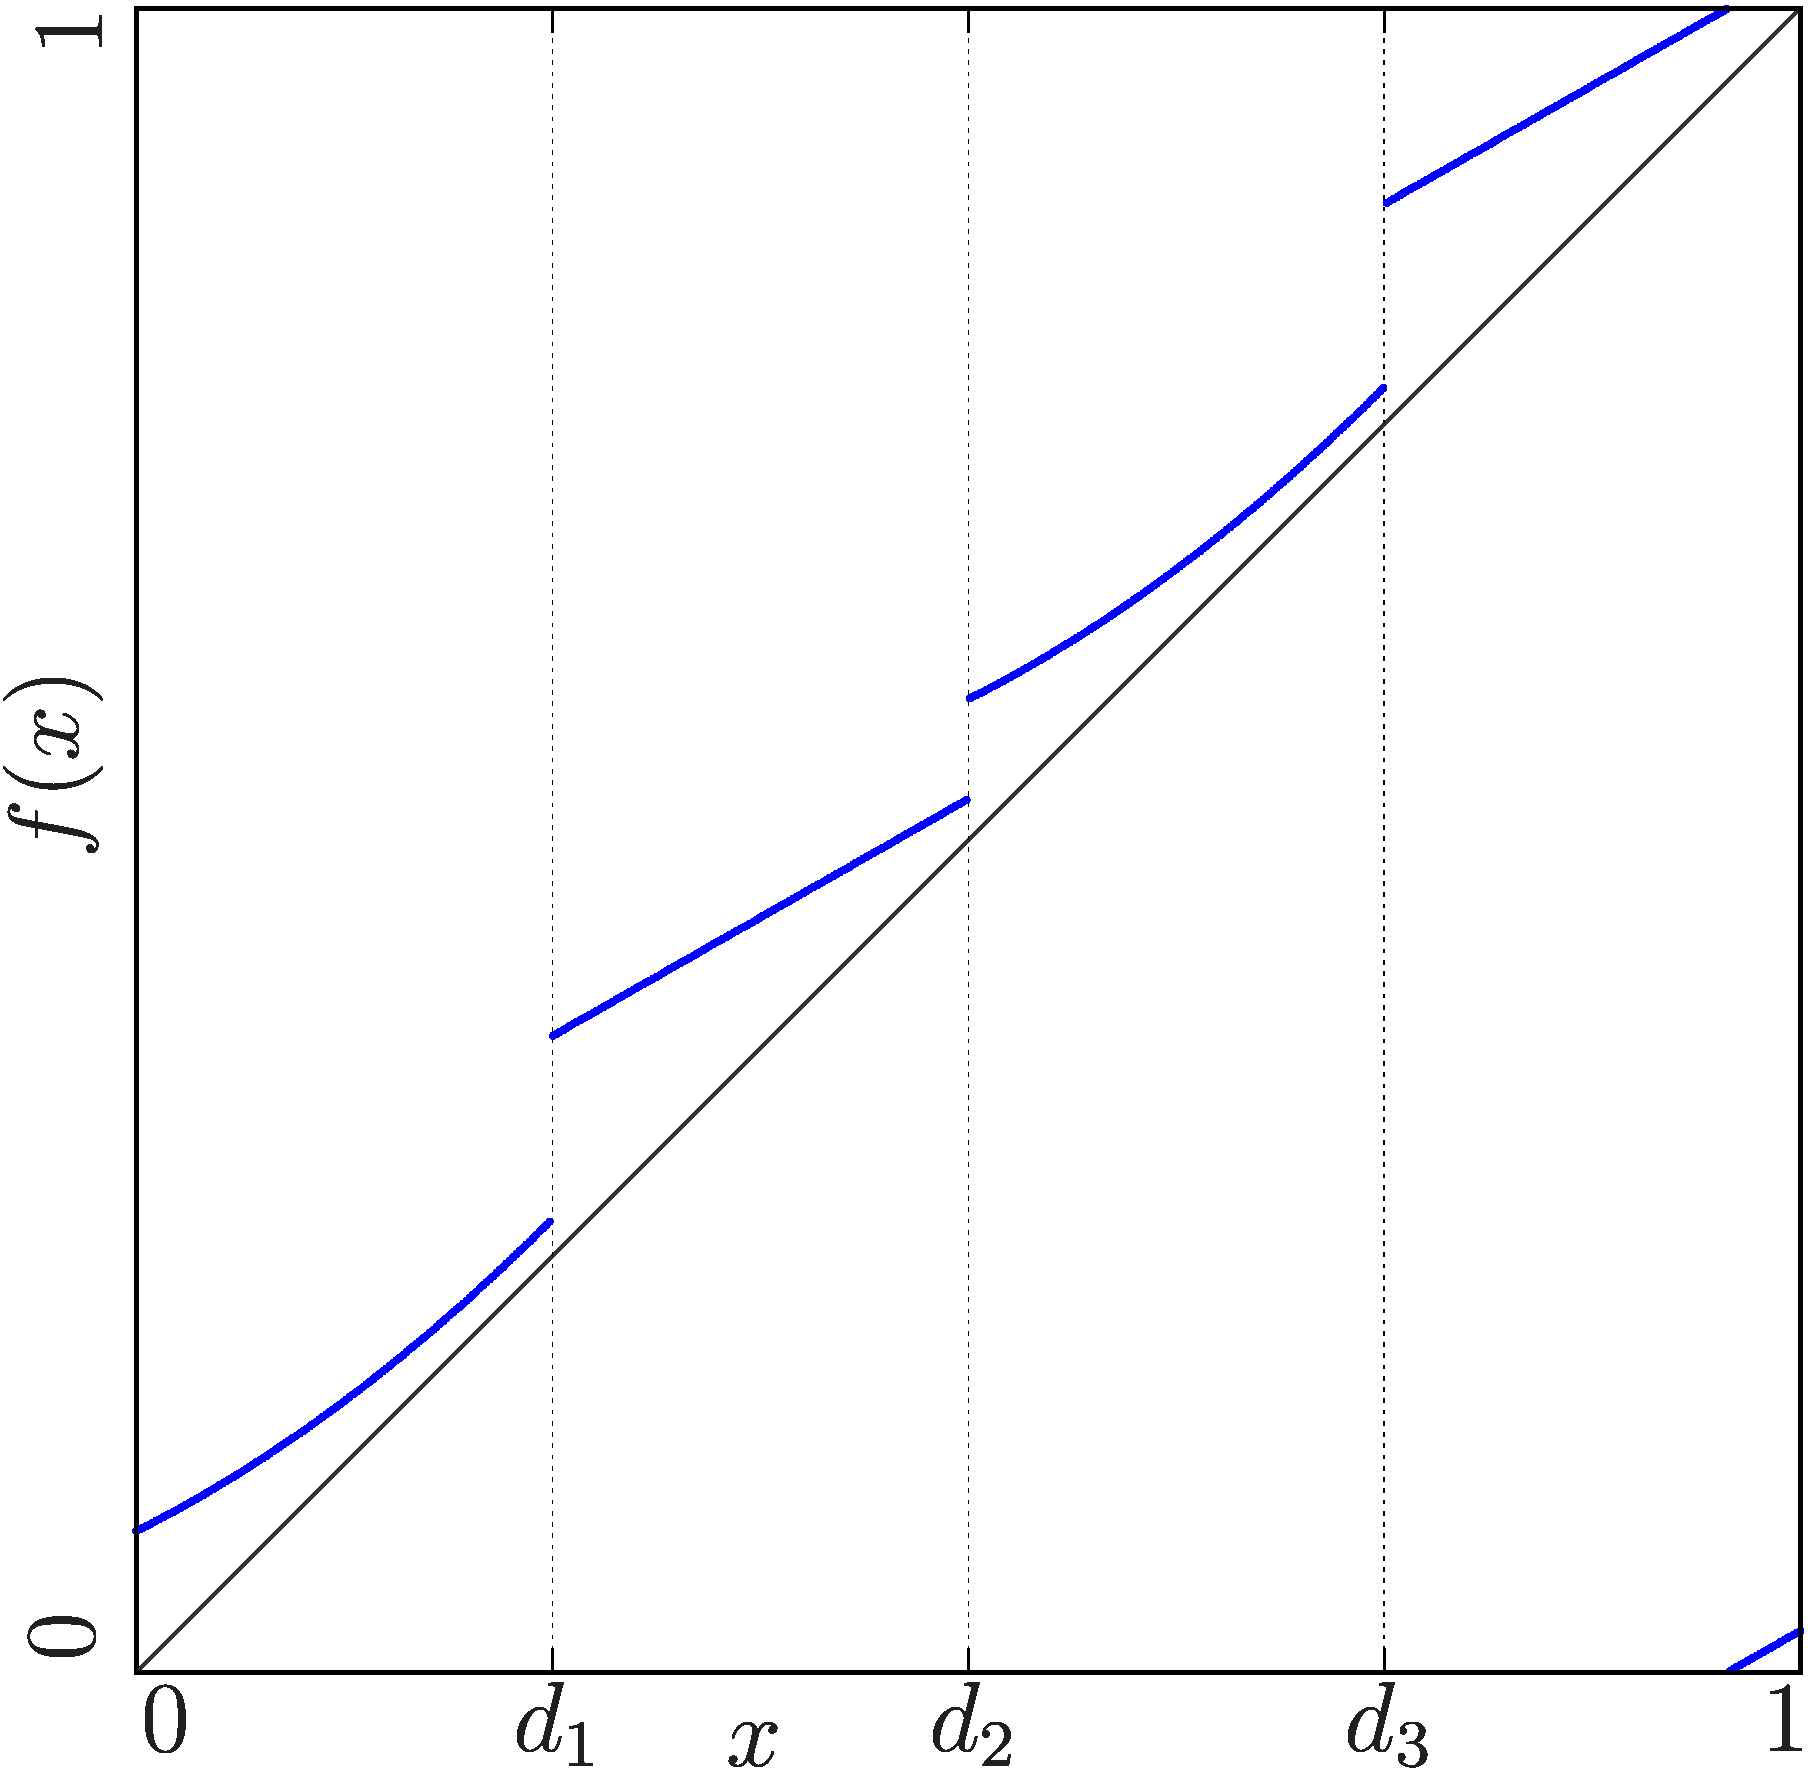
\includegraphics[width=.4 \textwidth]{../Figures/7/7.2a/result.png}
		\label{fig:add.saw}
	}
	\subfloat[Function shape]{
		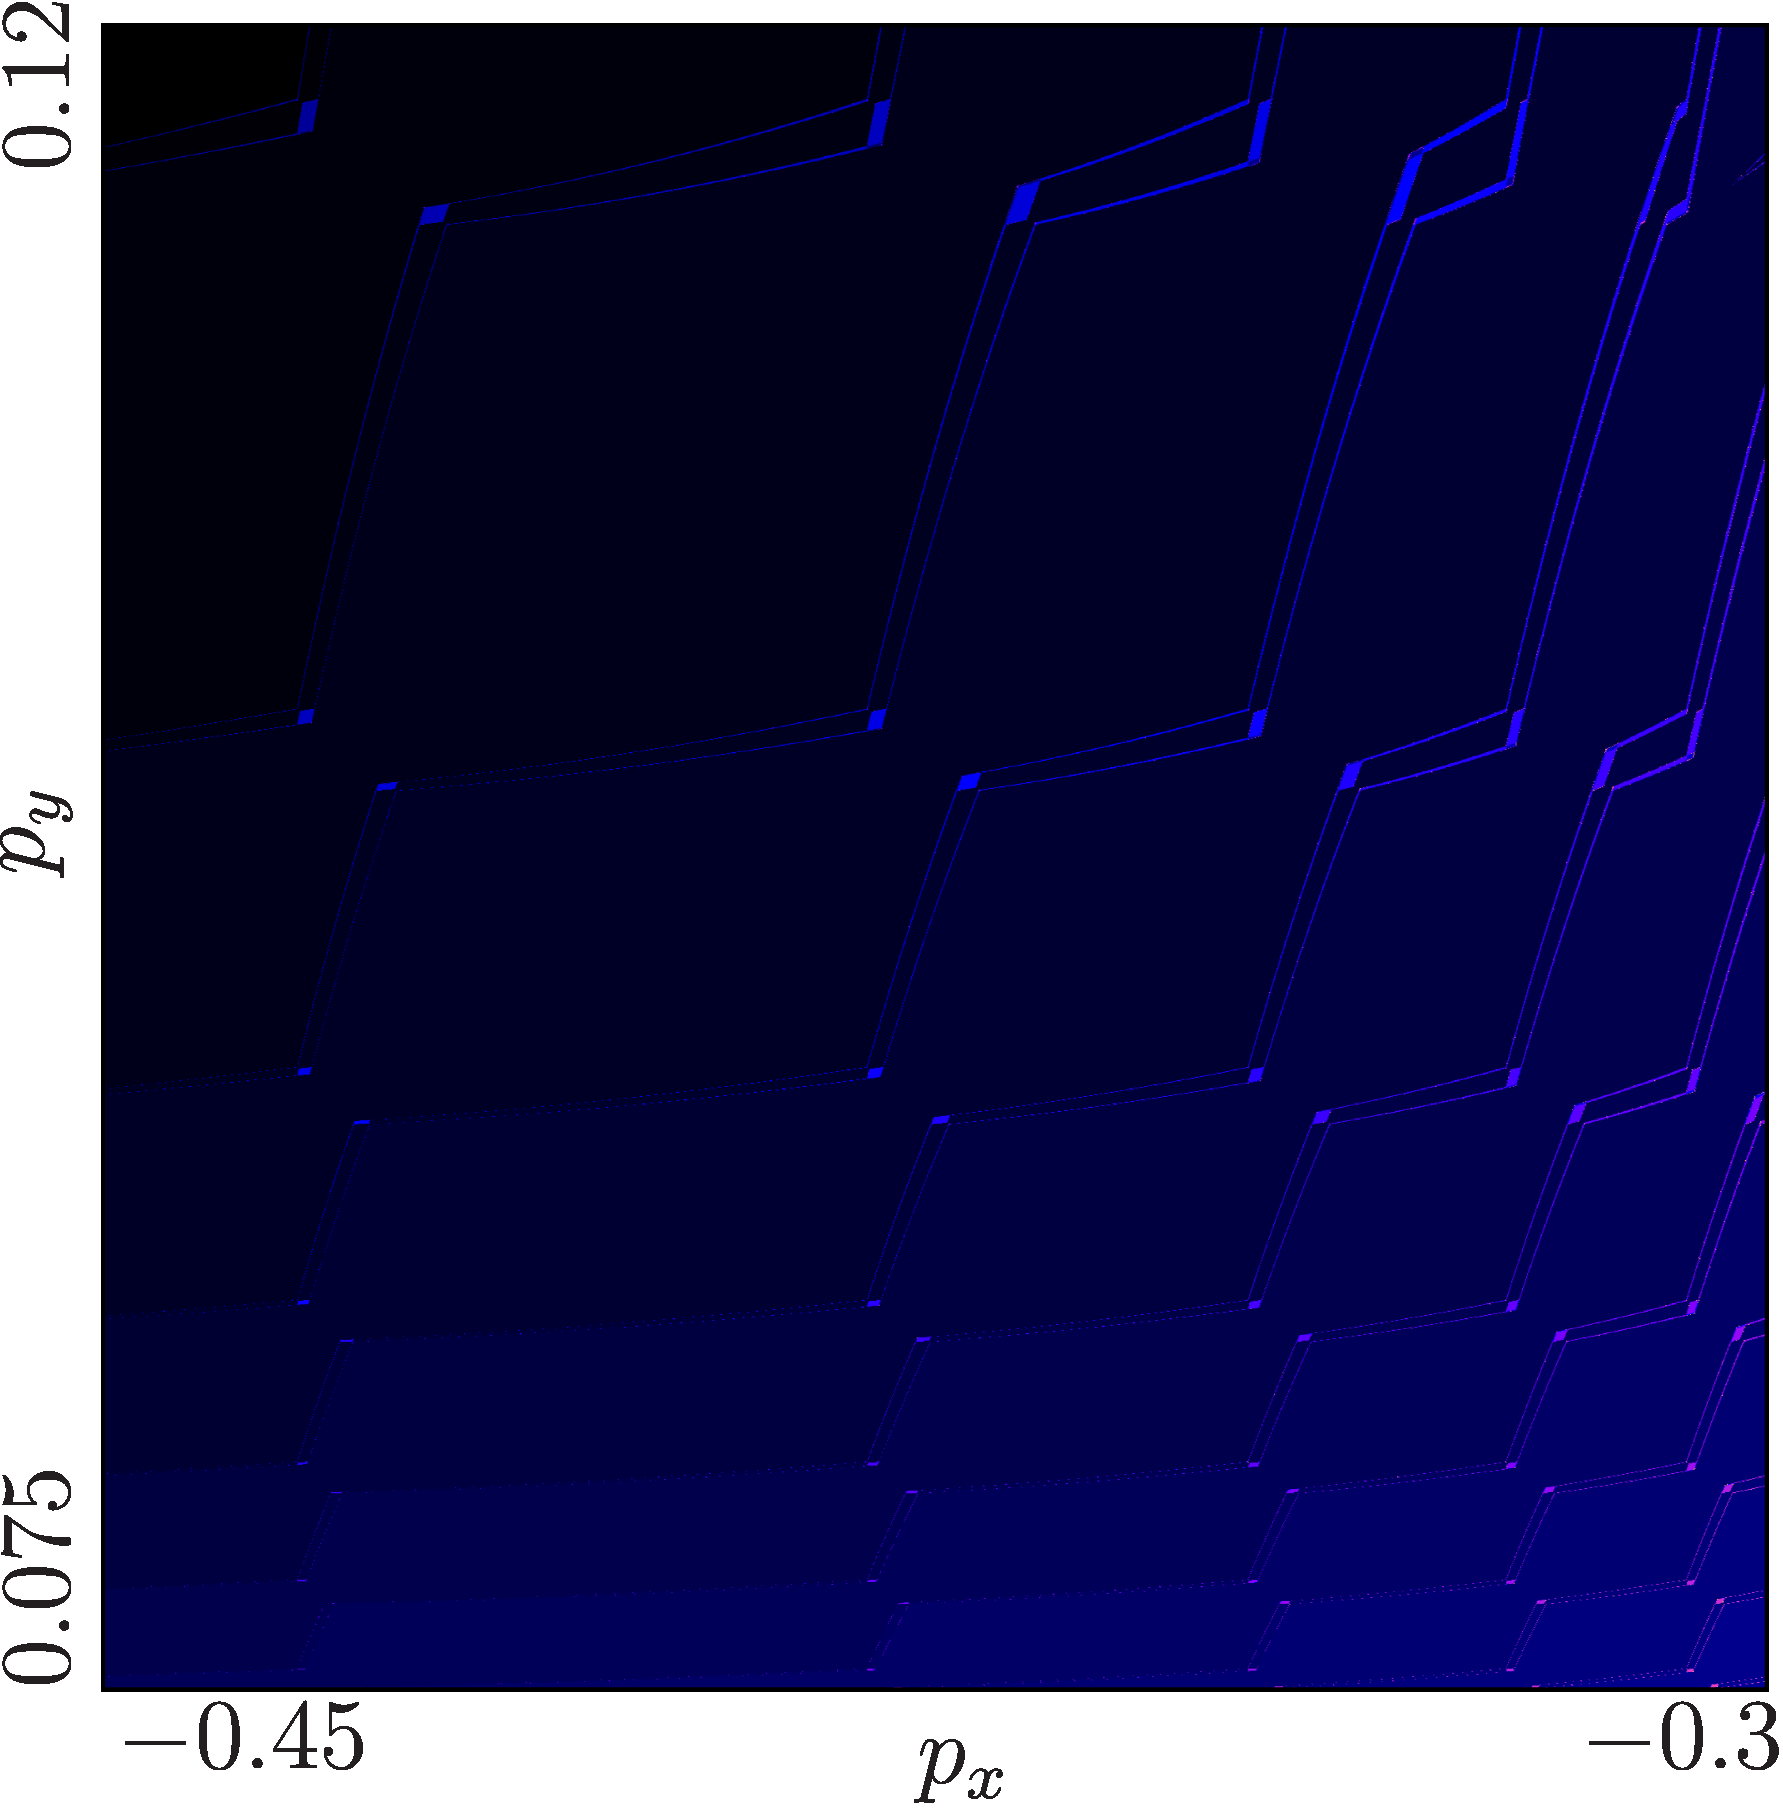
\includegraphics[width=.4 \textwidth]{../Figures/7/7.2b/result.png}
		\label{fig:add.arch.new}
	}
	\caption[Comparison of the piecewise-increasing archetypal model function and the skew sawtooth map]{
		Comparison of the piecewise-increasing archetypal model function and the skew sawtooth map.
		(a) shows the archetypal model function with the parameters $a_L = 1, b_L = \frac{1}{2}, c_L = 0.168, g_R\left(\frac{1}{4}\right) = -0.4 ,$ and $g_R\left(\frac{1}{2}\right) = \frac{1}{2} + \frac{1}{40}$.
		(b) shows the skew sawtooth map \hl{which is defined in} \cite{simpson2018saw} with the parameters $a_L = 0.5$ and $a_R = 1.5$.
		The parameters happen to have similar names to the parameters of the archetypal model.
	}
	\label{fig:add.saw.vs.arch}
\end{figure}
